%%%%%%%%%%%%%%%%%%%%%%%%%%%%%%%%%%%%%%%%%
% University Assignment Title Page 
% LaTeX Template
% Version 1.0 (27/12/12)
%
% This template has been downloaded from:
% http://www.LaTeXTemplates.com
%
% Original author:
% WikiBooks (http://en.wikibooks.org/wiki/LaTeX/Title_Creation)
%
% License:
% CC BY-NC-SA 3.0 (http://creativecommons.org/licenses/by-nc-sa/3.0/)
% 
% Instructions for using this template:
% This title page is capable of being compiled as is. This is not useful for 
% including it in another document. To do this, you have two options: 
%
% 1) Copy/paste everything between \begin{document} and \end{document} 
% starting at \begin{titlepage} and paste this into another LaTeX file where you 
% want your title page.
% OR
% 2) Remove everything outside the \begin{titlepage} and \end{titlepage} and 
% move this file to the same directory as the LaTeX file you wish to add it to. 
% Then add \input{./title_page_1.tex} to your LaTeX file where you want your
% title page.
%
%%%%%%%%%%%%%%%%%%%%%%%%%%%%%%%%%%%%%%%%%
%\title{Title page with logo}
%----------------------------------------------------------------------------------------
%	PACKAGES AND OTHER DOCUMENT CONFIGURATIONS
%----------------------------------------------------------------------------------------

\documentclass[12pt]{article}
\usepackage[english]{babel}
\usepackage[utf8x]{inputenc}
\usepackage{amsmath}
\usepackage{graphicx}
\usepackage{hyperref}
\usepackage[colorinlistoftodos]{todonotes}
\usepackage{geometry}
\geometry{left=3.8cm,right=3.8cm,top=2.5cm,bottom=2.5cm}

\begin{document}

\begin{titlepage}

\newcommand{\HRule}{\rule{\linewidth}{0.5mm}} % Defines a new command for the horizontal lines, change thickness here

\center % Center everything on the page
 
%----------------------------------------------------------------------------------------
%	HEADING SECTIONS
%----------------------------------------------------------------------------------------

\textsc{\LARGE Shanghai JiaoTong University}\\[1.5cm] % Name of your university/college
\textsc{\Large Data Mining}\\[0.5cm] % Major heading such as course name
\textsc{\large EE359}\\[0.5cm] % Minor heading such as course title

%----------------------------------------------------------------------------------------
%	TITLE SECTION
%----------------------------------------------------------------------------------------

\HRule \\[0.4cm]
{ \huge \bfseries Data Mining Final Project}\\[0.4cm] % Title of your document
\HRule \\[1.5cm]
 
%----------------------------------------------------------------------------------------
%	AUTHOR SECTION
%----------------------------------------------------------------------------------------

\begin{minipage}{0.4\textwidth}
\begin{flushleft} \large
\emph{Author:}\\
Yuting \textsc{Jia} % Your name
\end{flushleft}
\end{minipage}
~
\begin{minipage}{0.4\textwidth}
\begin{flushright} \large
\emph{Supervisor:} \\
Dr. Yuan \textsc{Bo} % Supervisor's Name
\end{flushright}
\end{minipage}\\[2cm]

% If you don't want a supervisor, uncomment the two lines below and remove the section above
%\Large \emph{Author:}\\
%John \textsc{Smith}\\[3cm] % Your name

%----------------------------------------------------------------------------------------
%	DATE SECTION
%----------------------------------------------------------------------------------------

{\large \today}\\[2cm] % Date, change the \today to a set date if you want to be precise

%----------------------------------------------------------------------------------------
%	LOGO SECTION
%----------------------------------------------------------------------------------------


\includegraphics[width=3.2in, height=3.2in]{logo.png}\\[1cm] % Include a department/university logo - this will require the graphicx package
 
%----------------------------------------------------------------------------------------

\vfill % Fill the rest of the page with whitespace

\end{titlepage}


\begin{abstract}
Your abstract.
\end{abstract}

\section{Introduction}

Your introduction goes here! Some examples of commonly used commands and features are listed below, to help you get started.

If you have a question, please use the support box in the bottom right of the screen to get in touch. 

\section{Data Collection}
\label{sec:data-collection}
We collected two different types of data. The first one is collected from Wind, a financial data company. This part of data is about the price of stock. And the other one is the data which TA give us, about the trade of some future goods.

\subsubsection{Wind Data}
Wind Financial Terminal (WFT), an indispensable tool to tap into the Chinese financial market, provides the most complete data and information on the Chinese financial market, covering stocks, bonds, funds, indices, warrants, commodity futures, foreign exchanges, and the macro industry, for securities analysts, fund managers and other financial professionals. This enables you to obtain the most accurate, timely and complete 7x24x365 financial information.

WFT provides users several interface to collect financial data, including EXCEL, MATLAB, R, Python and some other programming language. In this project, we chose the python interface because python is very convenient and stable.

From this interface, we collected the price information in recent three years for \textbf{2467} stocks. By this data, easily we can figure the price trend for each stock, and Figure \ref{fig:trend} are some examples of the trend of price of some stocks in recent three years.

\begin{figure}
\centering
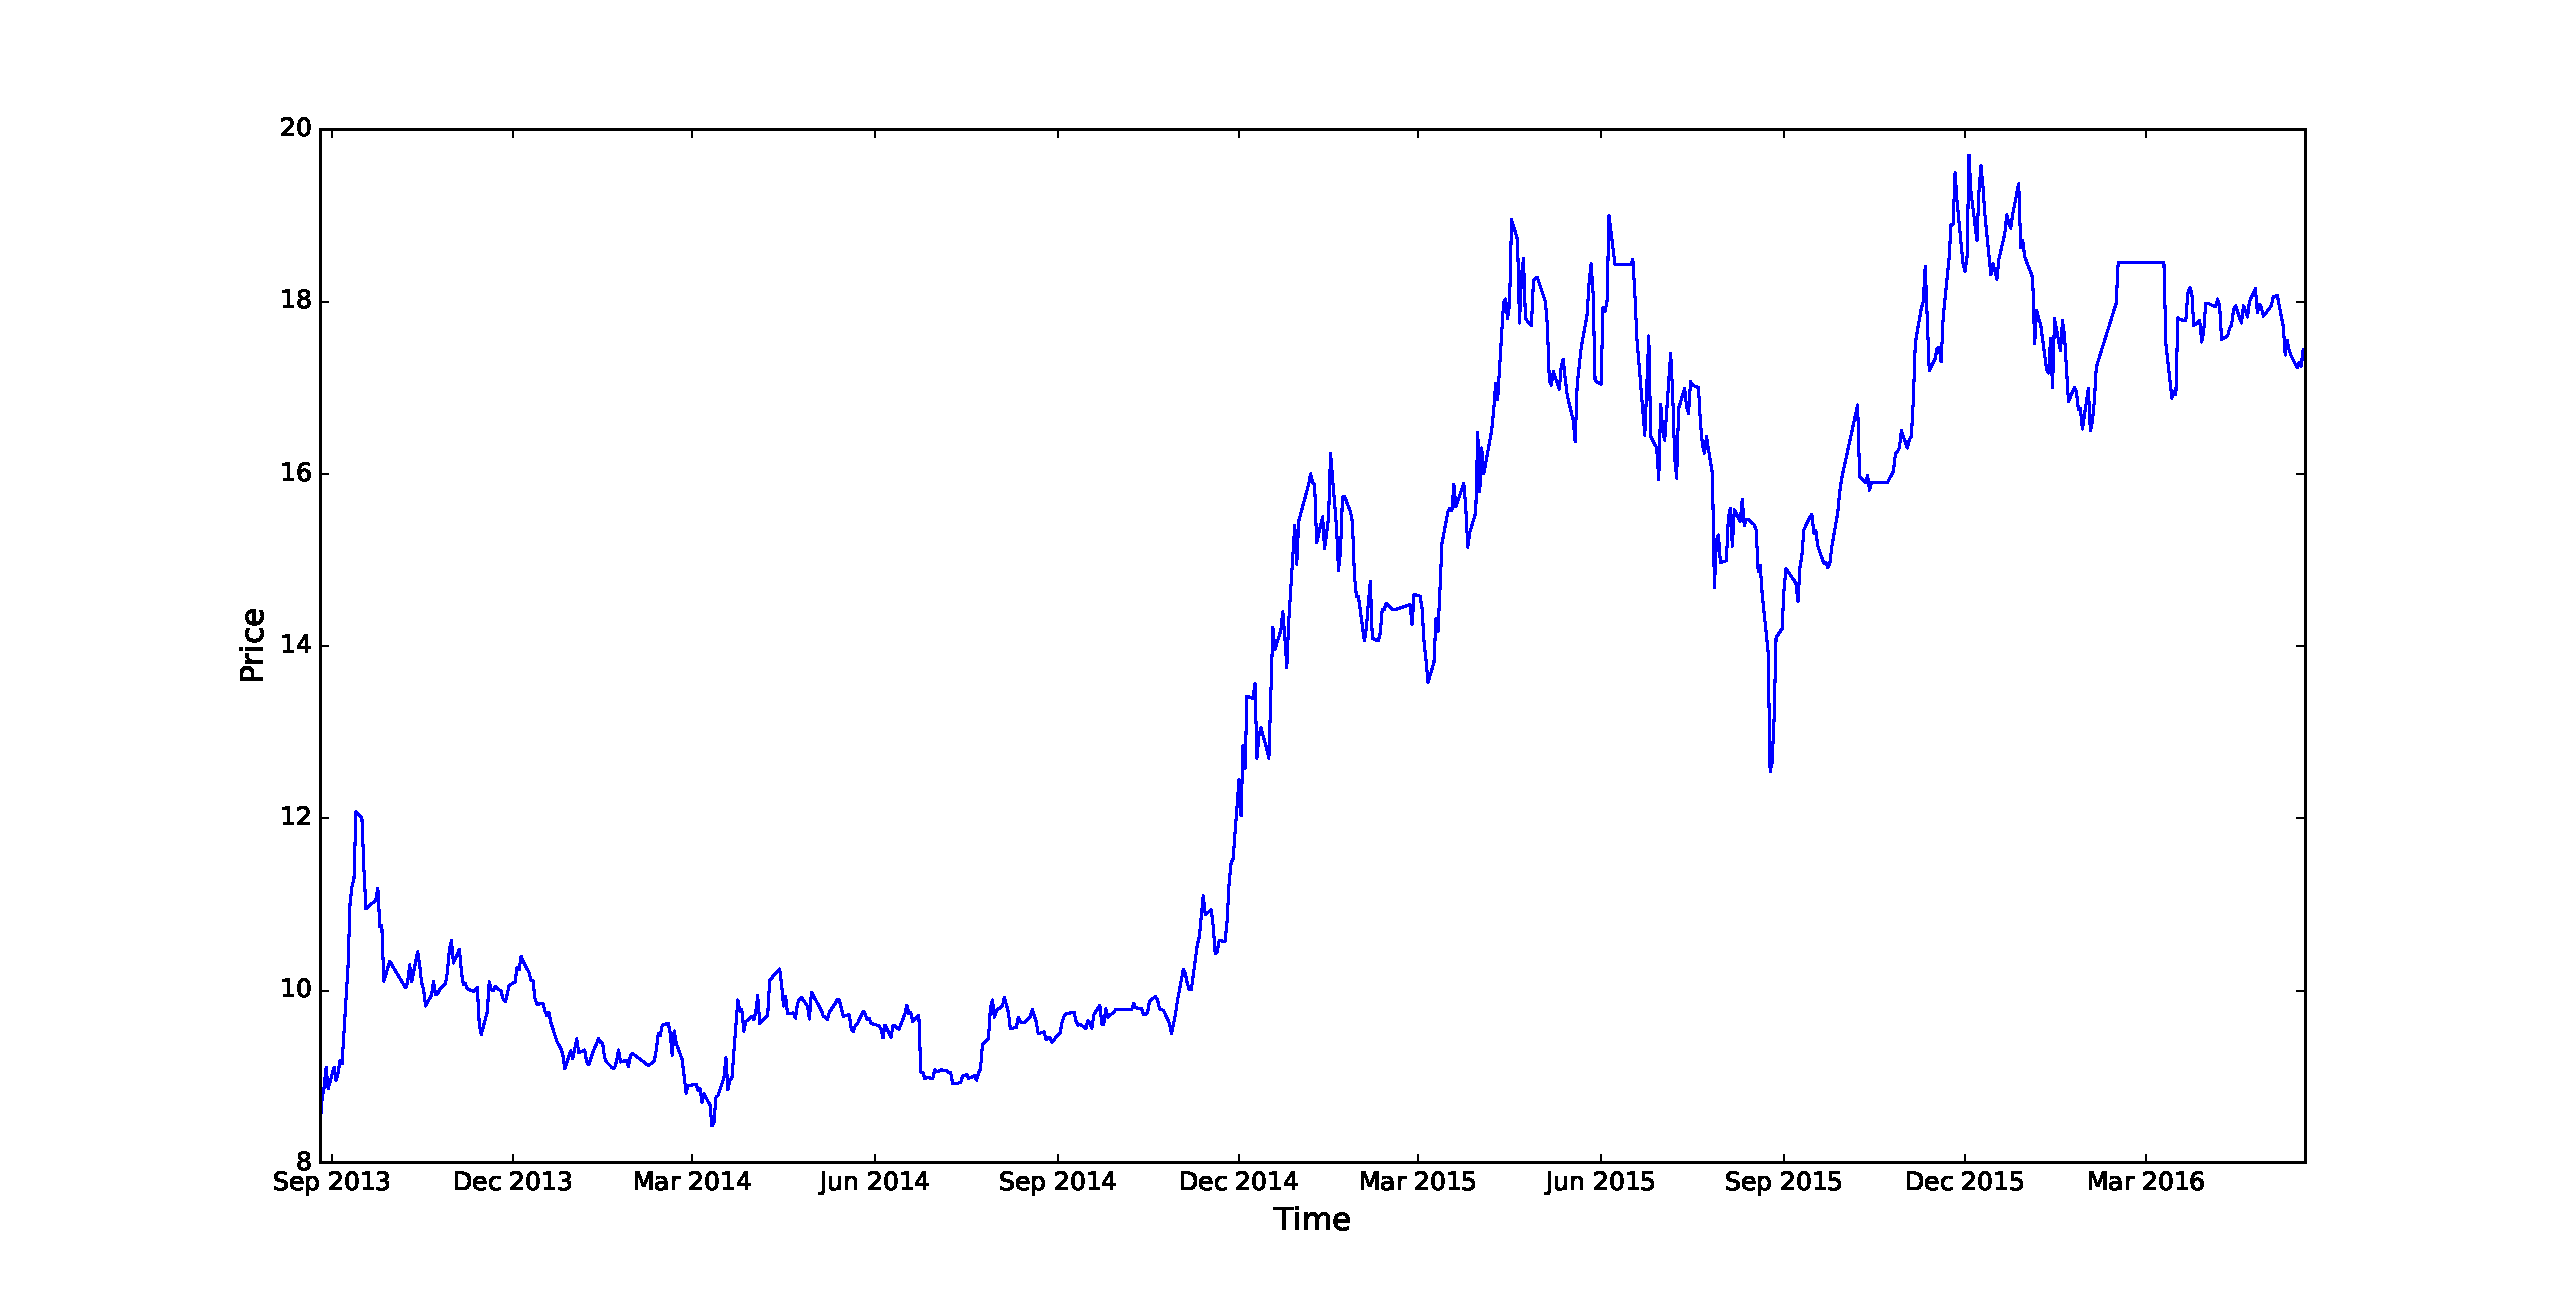
\includegraphics[width=1.0\textwidth]{trend1.pdf}
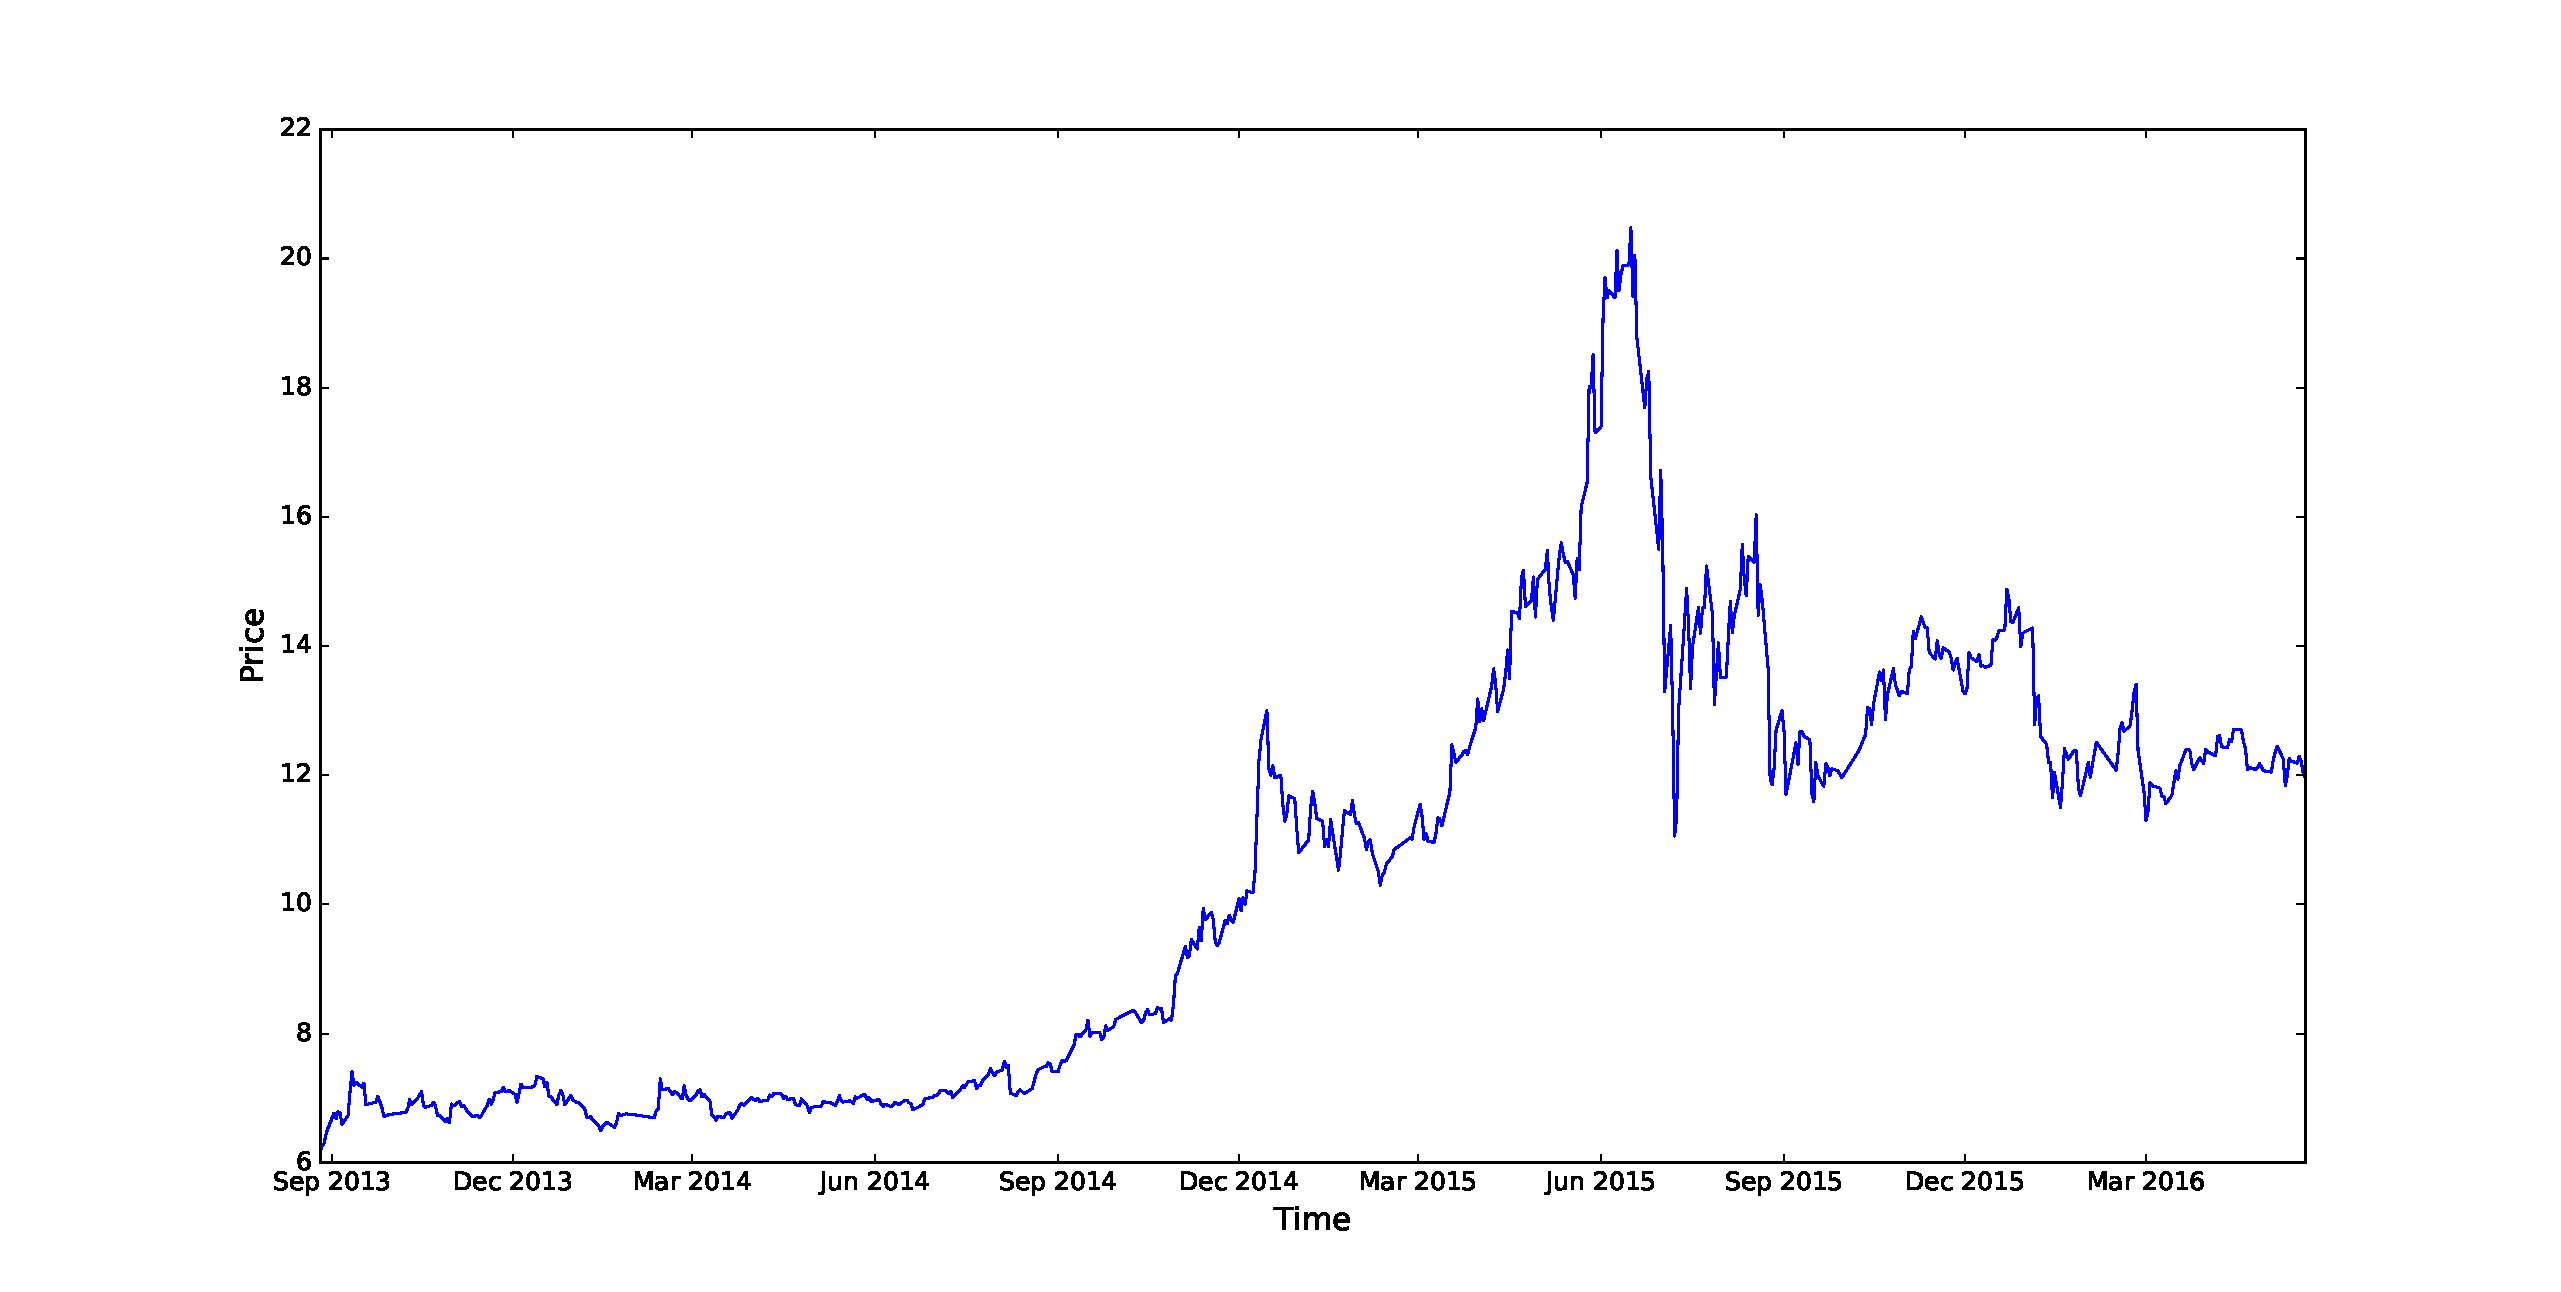
\includegraphics[width=1.0\textwidth]{trend2.pdf}
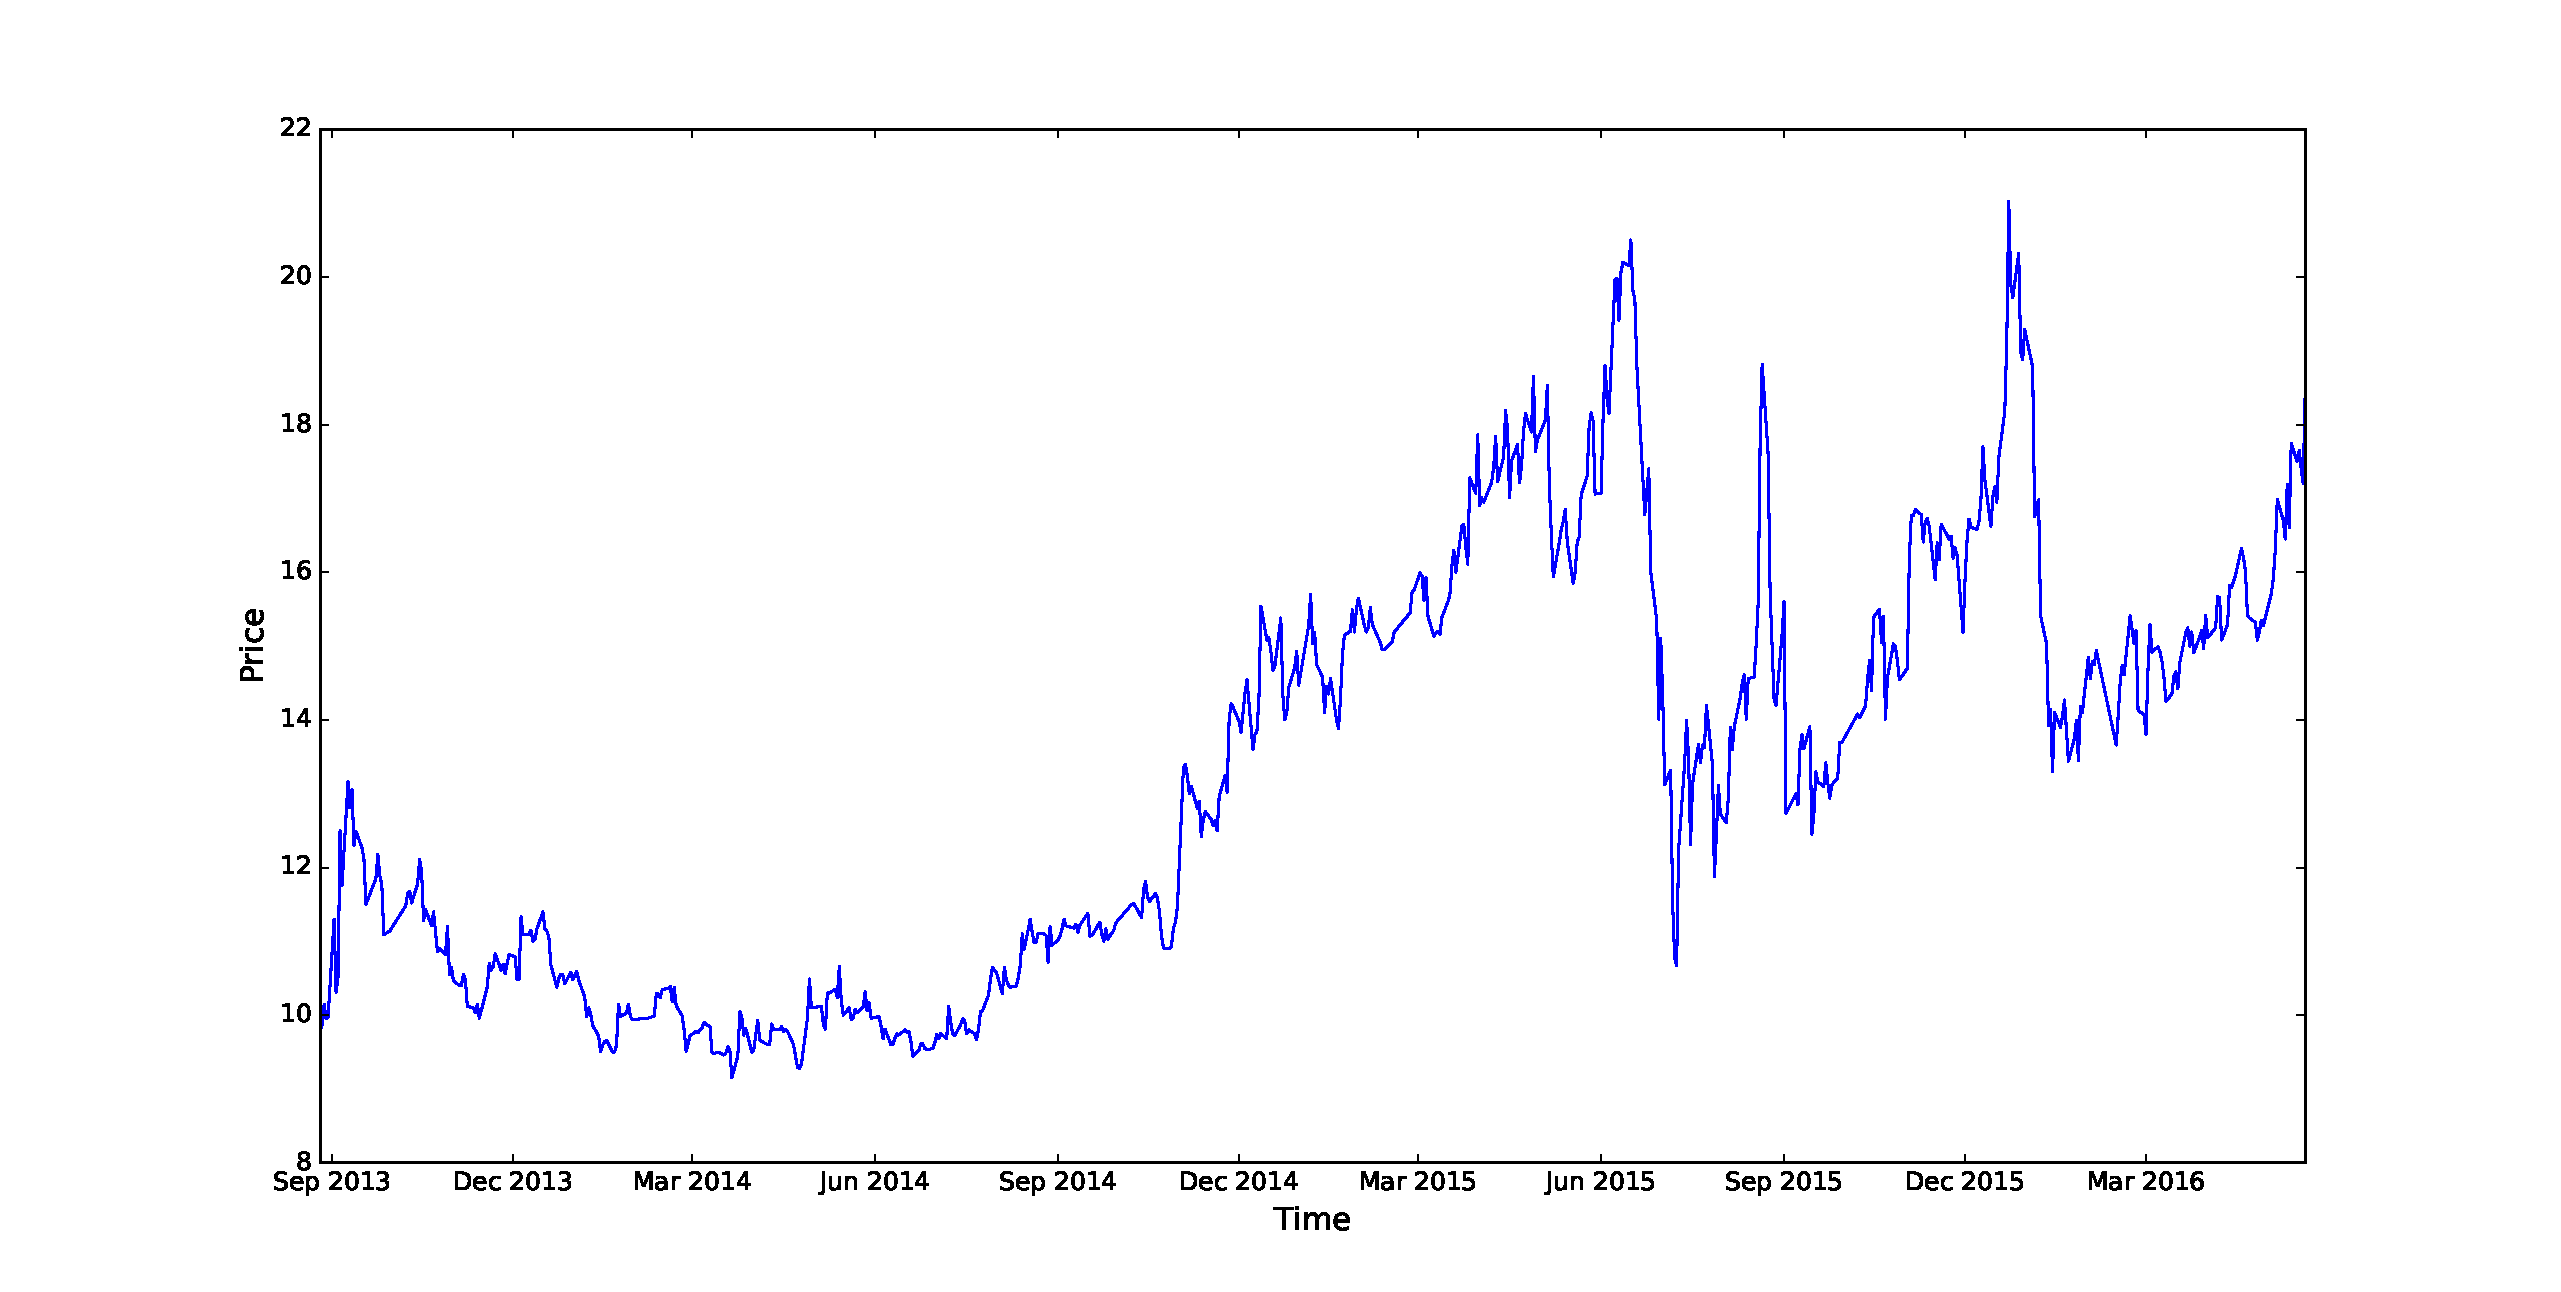
\includegraphics[width=1.0\textwidth]{trend3.pdf}
\caption{\label{fig:trend}Trend of price of some stocks}
\end{figure}

\subsubsection{Future Goods Trade}
This dataset is given by TA, including the trade record of several different future goods. According to TA, this dataset is enough for us to predict the price trend of future goods. And almost all exchange bourse are using this kind of data to predict future price and trade automatically.

\subsection{Experiments}
\subsubsection{Experiment 1}
Firstly we use the dataset collected from WFT. This dataset contains the open, close, highest and lowest price for each day. So the easiest and most intuitive thought is to use one day's four price to predict whether this stock rise up or fall down. So for each stock, we convert the four prices of each day to a vector, and use the trend of the second day as label(1 means rise up and -1 means fall down).

We decided to use SVM to learn this feature because it's useful, efficient and easy to realize. For each stock, we randomly chose 70\% percents of feature vectors as test set, and the other as test set. What's more, we think that different stock may hold different features, so we learn different SVM model for different stock respectively. Because we has 2467 stocks, so we count and print the cumulated accuracy rate for every 10 stocks. Figure \ref{fig:accuracy1} shows the change of accuracy rate with the number of stocks we have learned increase. We can find the the accuracy is about 53\%, just a little higher than randomly choose because this is a binary classification problem.

\begin{figure}
\centering
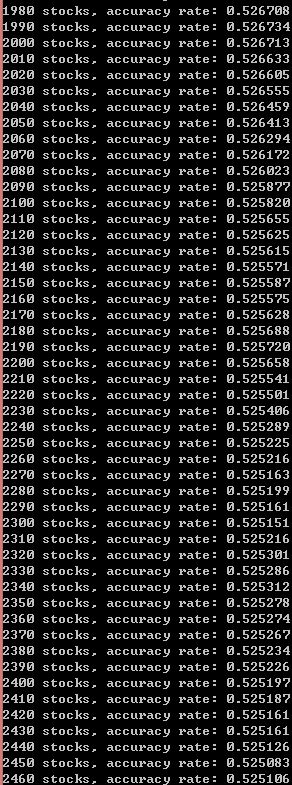
\includegraphics[width=0.5\textwidth]{accuracy1.png}
\caption{\label{fig:accuracy1}Change of Accuracy}
\end{figure}

This results is not beyond our expection. Because the method to extract features is so easy that cannot contain much hidden information of this financial market. And following we will try some other complex and meaningful methods to extract some more useful features.

\subsubsection{Experiment 2}
The data we collected is a timing series data. But in the former one experiment, we only use one day's data to predict the next day's trend. But the result is not very well. So now we come up with another thought that we can use data of several days to predict the following day's price. So now we use the continuous 5 days' price as the feature vector, and the label is just same with the label in the former experiment.

\begin{figure}
\centering
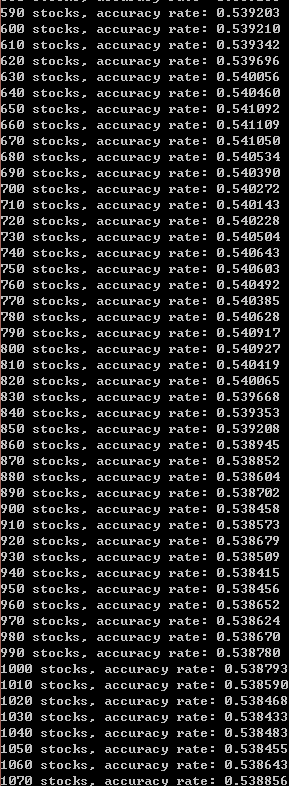
\includegraphics[width=0.5\textwidth]{accuracy2.png}
\caption{\label{fig:accuracy2}Change of Accuracy}
\end{figure}

Figure \ref{fig:accuracy2} shows the result of this experiment. From this figure we can find that the result is a little better than the former experiment, but the result is neither good enough. We think there are two reasons. The first one is that the time region we selected is not suitable. We chose to use five days' data to predict the following one day. But the region of five days can not express neither the instantaneous vibration nor the long-term trend of financial market. So the accuracy of the prediction is so low. The other one reason is that in this experiment we only use the close price of each day, so finally we also only used 5 number to be a feature vector, so the information in the feature is not enough.

\subsubsection{Experiment 3}
Because the time region of 5 days is not suitable, so we started to predict a long-term trend of the market. We start to combine each 5 days in one week to be one time-stamp and use five weeks of data to predict the trend of the next week. Unfortunately, this time the final accuracy is also about 54\%, which equals to the last experiment. This result means that actually we cannot only use price to predict price. What's more, if we think about the real financial market, we can find that the price of one stock in the last some week cannot mean anything. And it's price will only be affected by some other informations like the global financial state or some other news, but not only the price. So now we think that using price to predict price can not success.

\subsubsection{Experiment 4}
By WFT, we can only get the price data. But only use these informations is not enough, so we start to use the dataset provided by TA. In the dataset provided by TA, there are some record of the price provided by consumers and sellers. So by this information we can know the detailed process of the trade, showed in Figure \ref{fig:luowen1}. And we think we can use the process of trade to predict the price of the following trade.

\begin{figure}
\centering
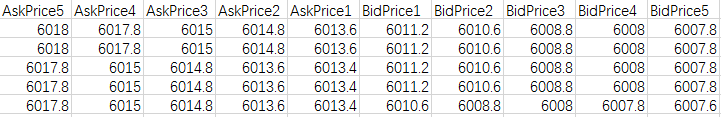
\includegraphics[width=1.0\textwidth]{luowen1.png}
\caption{\label{fig:luowen1}Dataset of Future Goods}
\end{figure}

From Figure \ref{fig:luowen1}, we can know the trend of the price provided by sellers and consumers respectively. And the change of price in this process can tell us the trend of the price of the future goods. So we count the number of rise up and fall down for each price as features and continue to use whether the price rise up as label. But this time is a little different, because we focus on twice adjacent trades, in which price often stay stable and do not change. So this time we has three labels, 1 means rise up, -1 means fall down and 0 means stay same. 

Figure \ref{fig:luowen2} shows the result of this classification problem. We can see that in most occasions, the accuracy is greater than 50\%. Please remember that this time the problem is a three-classification problem. So the accuracy of 50\% is much greater then 33\% and much better than the result we got in the former experiments.

\begin{figure}
\centering
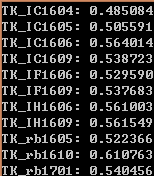
\includegraphics[width=0.5\textwidth]{luowen2.png}
\caption{\label{fig:luowen2}Accuracy of Prediction of Future Goods}
\end{figure}

\subsection{Sections}

Use section and subsection commands to organize your document. \LaTeX{} handles all the formatting and numbering automatically. Use ref and label commands for cross-references.

\subsection{Comments}

Comments can be added to the margins of the document using the \todo{Here's a comment in the margin!} todo command, as shown in the example on the right. You can also add inline comments too:

\todo[inline, color=green!40]{This is an inline comment.}

\subsection{Tables and Figures}

Use the table and tabular commands for basic tables --- see Table~\ref{tab:widgets}, for example. You can upload a figure (JPEG, PNG or PDF) using the files menu. To include it in your document, use the includegraphics command as in the code for Figure~\ref{fig:frog} below.

% Commands to include a figure:
\begin{figure}
\centering
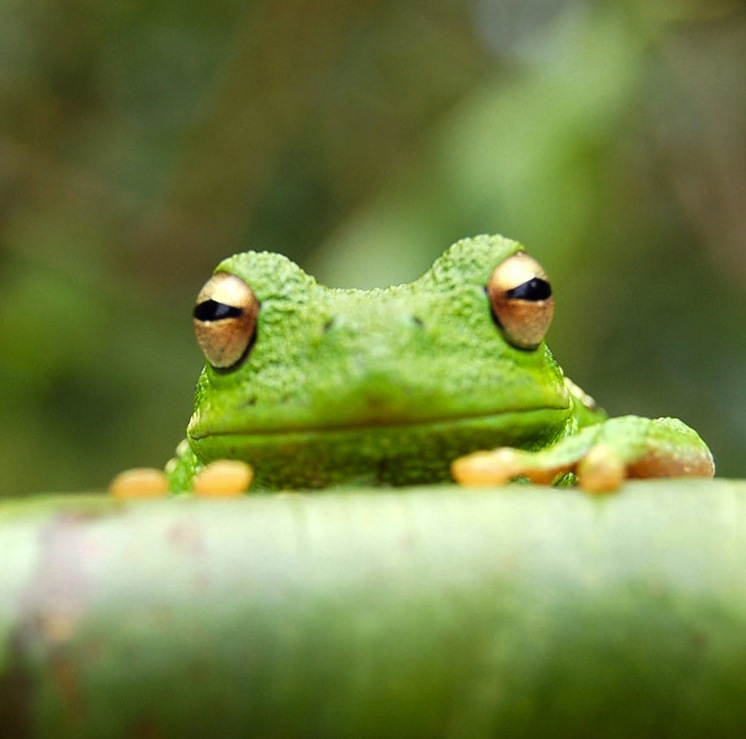
\includegraphics[width=0.5\textwidth]{frog.jpg}
\caption{\label{fig:frog}This is a figure caption.}
\end{figure}

\begin{table}
\centering
\begin{tabular}{l|r}
Item & Quantity \\\hline
Widgets & 42 \\
Gadgets & 13
\end{tabular}
\caption{\label{tab:widgets}An example table.}
\end{table}

\subsection{Mathematics}

\LaTeX{} is great at typesetting mathematics. Let $X_1, X_2, \ldots, X_n$ be a sequence of independent and identically distributed random variables with $\text{E}[X_i] = \mu$ and $\text{Var}[X_i] = \sigma^2 < \infty$, and let
$$S_n = \frac{X_1 + X_2 + \cdots + X_n}{n}
      = \frac{1}{n}\sum_{i}^{n} X_i$$
denote their mean. Then as $n$ approaches infinity, the random variables $\sqrt{n}(S_n - \mu)$ converge in distribution to a normal $\mathcal{N}(0, \sigma^2)$.

\subsection{Lists}

You can make lists with automatic numbering \dots

\begin{enumerate}
\item Like this,
\item and like this.
\end{enumerate}
\dots or bullet points \dots
\begin{itemize}
\item Like this,
\item and like this.
\end{itemize}

We hope you find write\LaTeX\ useful, and please let us know if you have any feedback using the help menu above.

\end{document}